% Options for packages loaded elsewhere
\PassOptionsToPackage{unicode}{hyperref}
\PassOptionsToPackage{hyphens}{url}
\PassOptionsToPackage{dvipsnames,svgnames*,x11names*}{xcolor}
%
\documentclass[
  11pt,
]{article}
\usepackage{lmodern}
\usepackage{amssymb,amsmath}
\usepackage{ifxetex,ifluatex}
\ifnum 0\ifxetex 1\fi\ifluatex 1\fi=0 % if pdftex
  \usepackage[T1]{fontenc}
  \usepackage[utf8]{inputenc}
  \usepackage{textcomp} % provide euro and other symbols
\else % if luatex or xetex
  \usepackage{unicode-math}
  \defaultfontfeatures{Scale=MatchLowercase}
  \defaultfontfeatures[\rmfamily]{Ligatures=TeX,Scale=1}
\fi
% Use upquote if available, for straight quotes in verbatim environments
\IfFileExists{upquote.sty}{\usepackage{upquote}}{}
\IfFileExists{microtype.sty}{% use microtype if available
  \usepackage[]{microtype}
  \UseMicrotypeSet[protrusion]{basicmath} % disable protrusion for tt fonts
}{}
\makeatletter
\@ifundefined{KOMAClassName}{% if non-KOMA class
  \IfFileExists{parskip.sty}{%
    \usepackage{parskip}
  }{% else
    \setlength{\parindent}{0pt}
    \setlength{\parskip}{6pt plus 2pt minus 1pt}}
}{% if KOMA class
  \KOMAoptions{parskip=half}}
\makeatother
\usepackage{xcolor}
\IfFileExists{xurl.sty}{\usepackage{xurl}}{} % add URL line breaks if available
\IfFileExists{bookmark.sty}{\usepackage{bookmark}}{
\usepackage{hyperref}
}
\hypersetup{
  pdftitle={TP2 système, shell},
  pdfauthor={Première NSI, Lycée du Parc},
  colorlinks=true,
  linkcolor=Maroon,
  filecolor=Maroon,
  citecolor=Blue,
  urlcolor=Blue,
  pdfcreator={LaTeX via pandoc}}
\urlstyle{same} % disable monospaced font for URLs
\usepackage[top=20mm,left=20mm,right=20mm,heightrounded]{geometry}
\usepackage{longtable,booktabs}
% Correct order of tables after \paragraph or \subparagraph
\usepackage{etoolbox}
\makeatletter
\patchcmd\longtable{\par}{\if@noskipsec\mbox{}\fi\par}{}{}
\makeatother
% Allow footnotes in longtable head/foot
\IfFileExists{footnotehyper.sty}{\usepackage{footnotehyper}}{\usepackage{footnote}}
\makesavenoteenv{longtable}
\usepackage{graphicx}
\makeatletter
\def\maxwidth{\ifdim\Gin@nat@width>\linewidth\linewidth\else\Gin@nat@width\fi}
\def\maxheight{\ifdim\Gin@nat@height>\textheight\textheight\else\Gin@nat@height\fi}
\makeatother
% Scale images if necessary, so that they will not overflow the page
% margins by default, and it is still possible to overwrite the defaults
% using explicit options in \includegraphics[width, height, ...]{}
\setkeys{Gin}{width=\maxwidth,height=\maxheight,keepaspectratio}
% Set default figure placement to htbp
\makeatletter
\def\fps@figure{htbp}
\makeatother
\setlength{\emergencystretch}{3em} % prevent overfull lines
\providecommand{\tightlist}{%
  \setlength{\itemsep}{0pt}\setlength{\parskip}{0pt}}
\setcounter{secnumdepth}{5}

\title{TP2 système, shell}
\usepackage{etoolbox}
\makeatletter
\providecommand{\subtitle}[1]{% add subtitle to \maketitle
  \apptocmd{\@title}{\par {\large #1 \par}}{}{}
}
\makeatother
\subtitle{Thème architectures matérielles et systèmes d'exploitation}
\author{Première NSI, \href{https://frederic-junier.org/}{Lycée du Parc}}
\date{}

%%%jolis boites

\usepackage{fancybox, graphicx}



%%%%%%%%%%%%%%%%Packages et Macros Frederic%%%%%%%%%%%%%%%%%%%%%%%%%%%%%


%%%%Insertion de liens hypertextes %%%%

            
%%%%%%%%%%PSTricks%%%%%%%%%%%%

\usepackage{pstricks,pst-plot,pst-text,pst-tree,pst-eps,pst-fill,pst-node,pst-math,pstricks-add,pst-xkey,pst-eucl}


%%%%%%%Tikz%%%%%%%%%%%%%%%
\usepackage{pgf,tikz,tkz-tab}
% Pour les tableaux de signes ou de variations avec tkz-tab voir https://zestedesavoir.com/tutoriels/439/des-tableaux-de-variations-et-de-signes-avec-latex/#1-13389_tikz-un-package-qui-en-a-dans-le-ventre
\usetikzlibrary{arrows}
\usetikzlibrary{shapes.geometric}
\usetikzlibrary{shapes.geometric}
\usetikzlibrary{petri}
\usetikzlibrary{decorations}
\usetikzlibrary{arrows}
\usetikzlibrary{math}
 %Variables must be declared in a tikzmath environment but
       % can be used outside
%       \tikzmath{int \n; \n = 508; \x1 = 1; \y1 =1; 
%                   %computations are also possible
%                    \x2 = \x1 + 1; \y2 =\y1 +3; } 


%%%%%%%%%%%%%%%%%%%%%%%%%%%%%%%%%%%%%%%%
%%%%%%%%%%%Commandes Tikz Perso%%%%%%%%%%%%%%%

% Définition des nouvelles options xmin, xmax, ymin, ymax
% Valeurs par défaut : -3, 3, -3, 3
\tikzset{
xmin/.store in=\xmin, xmin/.default=-3, xmin=-3,
xmax/.store in=\xmax, xmax/.default=3, xmax=3,
ymin/.store in=\ymin, ymin/.default=-3, ymin=-3,
ymax/.store in=\ymax, ymax/.default=3, ymax=3,
}
% Commande qui trace la grille entre (xmin,ymin) et (xmax,ymax)
\newcommand {\grille}[2]
{\draw[help lines,black, thick] (\xmin,\ymin) grid[xstep=#1, ystep=#2] (\xmax,\ymax);}
% Commande \axes
\newcommand {\axes} {
\draw[->,very thick] (\xmin,0) -- (\xmax,0);
\draw[->,very thick] (0,\ymin) -- (0,\ymax);
\draw (0.95*\xmax, 0) node[above] {};
\draw (0, 0.95*\ymax) node[left] {};
}
% Commande qui limite l?affichage à (xmin,ymin) et (xmax,ymax)
\newcommand {\fenetre}
{\clip (\xmin,\ymin) rectangle (\xmax,\ymax);}

%Exemple d'utilisation

%\begin{center}
%\begin{tikzpicture} [xmin=-2,xmax=2,ymin=0,ymax=5]
%\grille{1} \axes \fenetre
%\draw plot[smooth] (\x,\x^2);
%\end{tikzpicture}
%\end{center}

%style pour la perspective cavalière française
%voir Tikz pour l'impatient page 68
\tikzset{math3d/.style=
{x= {(-0.353cm,-0.353cm)}, z={(0cm,1cm)},y={(1cm,0cm)}}}

%%%%%%%Symbole pour code calculatrice%%%%%%

%Flèche remplie pour défilement de menu

\newcommand{\flechefillright}{

\begin{tikzpicture}[scale=0.15] \fill (0,0)--(2,1)--(0,2)--cycle;
\end{tikzpicture}}

%%%%%%%%%%%%%Symboles pour calculatrice Casio%%%%
\newcommand{\execasio}{\Pisymbol{psy}{191}} %Retour chariot
\newcommand{\dispcasio}{\begin{pspicture}(.1,.1)\pspolygon*(.1,0)(.1,.1)\end{pspicture}} %Triangle « Disp »
\newcommand{\dispcasiotikz}{
\begin{tikzpicture}[scale=0.2]
\fill (0,0) -- (1,0) -- (1,1) -- cycle;
\end{tikzpicture}} %Triangle « Disp »
%

%Fleche entre deux lignes, d'apres 'un bon petit' : http://forum.mathematex.net/latex-f6/fleches-entre-deux-lignes-pour-resolution-d-equation-t10283.html#p99817
\newcommand\addnode[1]{\Rnode{#1}{}}
\newcommand\linknode[3]{\ncbar[angleA=0,angleB=0,nodesep=1ex,arm=10ex,offset=-2pt]{->}{#1}{#2}\Aput{\vphantom{x}#3}}


%%Commande pour touche de calculatrice

\newcommand\tc[1]{%
{
\begin{tikzpicture}
\node[draw,rectangle,rounded corners=3pt] (P) at (0,0){#1};
\end{tikzpicture}
}
}

%%%%%%%%%%%%%%%%%%%%%%%%%%%%%%%%%%%%%%%%
%%%%%%%%%%%Fin Commandes Tikz%%%%%%%%%%%%%%%


%%%%%%%%%%%%Specifiques%%%%%%%%%%%
\usepackage{wrapfig}
%pour insérer une figure à droite ou à gauche d'un texte
%\begin{wrapfigure}[nb lignes]{placement l,r,c,i(inside),o(outside)}[overhang]{width}
%ce package fonctionne mal à proximité des listes
%%%%%%%%%%%%%%%%%%%%%%%%%%%%%%%%%%%%%

%%%%%Environnements et symboles spéciaux pour faire joli%%%%%%

%%%Bclogo, pour des environnements + jolis avec insertion de logo%%%%
%Dépendances de  bclogo
\usepackage{xkeyval}  
\usepackage{etoolbox}
\usepackage{ifpdf}
\usepackage[framemethod=tikz]{mdframed}
\usepackage[tikz]{bclogo}

%\newcommand\bcpython{\includegraphics[width=17pt]{/home/fjunier/Maths/python-logo.eps}}
\newcommand\bcpython{\includegraphics[width=17pt]{/home/fjunier/Maths/python-logo.png}}
%\newcommand\bcpython{\includegraphics[width=17pt]{/home/frederic/Maths/python-logo.png}}

%% Framed
\usepackage{framed}  %Le package « framed» Crée 3 nouveaux environnements, qui se comportent comme des minipage de largeur \linewidth, mais permettant en plus de se casser entre plusieurs pages.     * framed : avec un cadre autour;     * shaded : avec un fonc coloré (il faut définir la couleur shadecolor);     * leftbar : avec une barre le long du côté gauche.

%%%%%%%%%%%%%%%%%%%Présentation de codes sources%%%%%%%%%%%%%%%%%
\usepackage{listings}
%On utilise l?environnement lstlisting pour insérer
%un code source.
%En plus de l?environnement lstlisting, on peut également utiliser la
%commande \lstinline qui fonctionne comme la commande \verb, en ce
%sens qu?on peut utiliser n?importe quel caractère comme délimiteur. Enfin,
%la commande \lstinputlisting permet de charger un code source depuis
%un fichier externe.
%Il y a deux manières de préciser des options : soit via l?option de l?envi-
%ronnement ou de la commande, soit en utilisant la commande \lstset
%qui permet de définir des options de manière globale.

\lstset{ %
  language=Python,                % the language of the code
  basicstyle=\ttfamily,           % the size of the fonts that are used for the code
  %numbers=left,                   % where to put the line-numbers
  numberstyle=\tiny,  % the style that is used for the line-numbers
  %stepnumber=2,                   % the step between two line-numbers. If it's 1, each line 
                                  % will be numbered
  %numbersep=5pt,                  % how far the line-numbers are from the code
  backgroundcolor=\color{white},      % choose the background color. You must add \usepackage{color}
  showspaces=false,               % show spaces adding particular underscores
  showstringspaces=false,         % underline spaces within strings
  showtabs=false,                 % show tabs within strings adding particular underscores
  frame=single,                   % adds a frame around the code
  rulecolor=\color{black},        % if not set, the frame-color may be changed on line-breaks within not-black text (e.g. comments (green here))
  tabsize=4,                      % sets default tabsize to 2 spaces
  captionpos=b,                   % sets the caption-position to bottom
  breaklines=true,                % sets automatic line breaking
  breakatwhitespace=false,        % sets if automatic breaks should only happen at whitespace
  %title=\lstname,                   % show the filename of files included with \lstinputlisting;
                                  % also try caption instead of title
  breakindent=1cm,
  keywordstyle=\color{blue},          % keyword style
  commentstyle=\color{red},       % comment style
  %stringstyle=\ttfamily\color{green},         % string literal style
  escapeinside={\%*}{*)},            % if you want to add LaTeX within your code
  morekeywords={*,...},              % if you want to add more keywords to the set
  deletekeywords={...}              % if you want to delete keywords from the given language
  upquote=true,columns=flexible,
xleftmargin=1cm,xrightmargin=1cm,
 inputencoding=utf8,			%Les lignes qui suivent sont pour le codage utf8
  extendedchars=true,
  literate=%
            {é}{{\'{e}}}1
            {è}{{\`{e}}}1
            {ê}{{\^{e}}}1
            {ë}{{\¨{e}}}1
            {û}{{\^{u}}}1
            {ù}{{\`{u}}}1
            {â}{{\^{a}}}1
            {à}{{\`{a} }}1
            {î}{{\^{i}}}1
            {ô}{{\^{o}}}1
            {ç}{{\c{c}}}1
            {Ç}{{\c{C}}}1
            {É}{{\'{E}}}1
            {Ê}{{\^{E}}}1
            {À}{{\`{A}}}1
            {Â}{{\^{A}}}1
            {Î}{{\^{I}}}1
}

\lstdefinestyle{rond}{
  numbers=none,
  backgroundcolor=\color{gristclair},
  frameround =tttt
}

\lstdefinestyle{compil}{
  numbers=none,
  backgroundcolor=\color{gristclair}
}
%\lstset{language=Python,basicstyle=\small , frame=single,tabsize=4,showspaces=false,showtabs=false,showstringspaces=false,numbers=left,numberstyle=\tiny , extendedchars=true}



%%%%%%%%%%%%%%%%%%%%%%%%%%%%%%%%%%%%%%%%%%%%%%%%%%%%%%%%%%%%%%%%%%%%%%%%
%%%%%%%%%%%%%%%%%%%%Environnements persos%%%%%%%%%%%%%%%%%%%%%%%%%%%%%%%%
%Syntaxe :
%\newenvironment{nom}[nombre d'args][defaut]{definitions initiales}{definitions finales}
%definitions intiales sont les commandes appelées par \begin{nom}
%Definitions finales sont les commandes appelées par \end{nom}

%%%%%%%%%%%%%%%%Définitions des environnemts persostheoreme, exemple ..%%%%
%%%% Exercice avec encadré %%%%
\newcounter{exo}
\newenvironment{exercice}[1]
{\par \medskip   \addtocounter{exo}{1} \noindent  
\begin{bclogo}[arrondi =0.1,   noborder = true, logo=\bccrayon, marge=4]{~\textbf{Exercice} \textbf{\theexo} {\itshape #1} }  \par}
{
\end{bclogo}
 \par \bigskip }

%%Axiomes, Theoremes, Propriété, Définition, Methode, Preuve


\newenvironment{axiome}[1]
{\par \medskip   \begin{leftbar} \noindent \underline{\textbf{Axiome}}\hspace{0.5cm}{\itshape #1}   \vspace*{10pt} \par }
{\end{leftbar}  \par \medskip }


\newcounter{thme}
\newenvironment{theoreme}[1]
{\par \medskip  \addtocounter{thme}{1} \noindent  
\begin{bclogo}[arrondi =0.1,  ombre = true, barre=none, logo=\bcbook, marge=4]{~\textbf{Théorème} \textbf{\thethme} {\itshape #1} }   \par}
{
\end{bclogo}
 \par \bigskip}

 \newenvironment{theoremedef}[1]
{\par \medskip   \addtocounter{thme}{1} \noindent  
\begin{bclogo}[arrondi =0.1,  ombre = true, barre=none, logo=\bcbook, marge=4]{~\textbf{Théorème-Définition} \textbf{\thethme} {\itshape #1} }   \par}
{
\end{bclogo}
 \par \bigskip }
 
\newcounter{prop}
\newenvironment{propriete}[1]
{\par \medskip   \addtocounter{prop}{1} \noindent  
\begin{bclogo}[arrondi =0.1,  ombre = true, barre=none, logo=\bcbook, marge=4]{~\textbf{Propriété} \textbf{\theprop} {\itshape #1} }   \par}
{
\end{bclogo}
 \par \bigskip }


\newenvironment{corollaire}[1]
{\par \medskip   \noindent  
\begin{bclogo}[arrondi =0.1,  ombre = true, barre=none, logo=\bcbook, marge=4]{~\textbf{Corollaire} {\itshape #1} } \par }
{
\end{bclogo}
 \par \bigskip }

\newenvironment{demo}[1]
{\par \medskip   \noindent  
\begin{bclogo}[arrondi =0.1,  ombre = true, barre=zigzag, noborder = true, logo=\bcloupe, marge=0]{~\textbf{Démonstration} {\itshape #1} } \par \vspace{10pt}}
{
\end{bclogo}
 \par \bigskip }

\newcounter{activite}
\newenvironment{activite}[1]
{\par \medskip   \noindent   \addtocounter{activite}{1}
\begin{bclogo}[arrondi =0.1,   noborder = true, logo=\bcvelo, marge=4]{~\textbf{Activité} \textbf{\theactivite} {\itshape #1} }  \par}
{
\end{bclogo}
 \par \bigskip }


\newcounter{rque}
\newenvironment{remarque}
{\par \medskip    \addtocounter{rque}{1} \noindent  
\begin{bclogo}[arrondi =0.1,  ombre = true, barre=snake, noborder = true, logo=\bcinfo, marge=0]{~\textbf{Remarque} \textbf{\therque}}  \par }
{
\end{bclogo}
 \par \bigskip }

\newcounter{def}
\newenvironment{definition}[1]
{\par \medskip   \addtocounter{def}{1} \noindent  
\begin{bclogo}[arrondi =0.1,  ombre = true, barre=none, logo=\bcbook, marge=4]{~\textbf{Définition} \textbf{\thedef} {\itshape #1} }  \par}
{
\end{bclogo}
 \par \bigskip }
 
 
 \newcounter{cours}
\newenvironment{cours}[1]
{\par \medskip   \addtocounter{cours}{1} \noindent  
\begin{bclogo}[arrondi =0.1,  ombre = true, barre=none, logo=\bcbook, marge=4]{~\textbf{Point de cours} \textbf{\thecours} {\itshape #1} }  \par}
{
\end{bclogo}
 \par \bigskip }
 
 

\newenvironment{memo}[1]
{\par \medskip    \noindent  
\begin{bclogo}[arrondi =0.1,  ombre = true, barre=none, logo=\bccle, marge=4]{~\textbf{À retenir}  {\itshape #1} }  \par}
{
\end{bclogo}
 \par \bigskip }
 
\newcounter{exple}
\newenvironment{exemple}[1]
{\par \medskip   \addtocounter{exple}{1} \noindent  
\begin{bclogo}[arrondi =0.1,   noborder = true, logo=\bclampe, marge=4]{~\textbf{Exemple} \textbf{\theexple} {\itshape #1} }  \par}
{
\end{bclogo}
 \par \bigskip }




\newcounter{alg}
\newenvironment{algorithme}[1]
{\par \medskip   \addtocounter{alg}{1} \noindent  
 \begin {bclogo}[noborder = true, barre=zigzag,logo=\bcpython, marge=4] {~\textbf{Algorithmique} \textbf{\thealg} {\itshape #1} }  \par}
{
\end{bclogo}
 \par \bigskip }

\newcounter{prog}
\newenvironment{programme}[1]
{\par \medskip   \addtocounter{prog}{1} \noindent  
 \begin {bclogo}[noborder = true, barre=zigzag,logo=\bcpython, marge=4] {~\textbf{Programme} \textbf{\theprog} {\itshape #1} }  \par  \bigskip}
{
\end{bclogo}
 \par \bigskip }
 
\newcounter{logi}
\newenvironment{logique}[1]
{\par \medskip   \addtocounter{logi}{1} \noindent  
 \begin {bclogo}[noborder = true, barre=zigzag,logo=\bclampe, marge=4] {~\textbf{Logique} \textbf{\thelogi} {\itshape #1} }  \par}
{
\end{bclogo}
 \par \bigskip }


\newenvironment{methode}[1]
{\par \medskip    \noindent  
 \begin {bclogo}[arrondi =0.1,logo=\bcoutil, marge=4,noborder = true] {~\textbf{Méthode}   {\itshape #1} }  \par}
{
\end{bclogo}
 \par \bigskip }


\newcounter{histo}
\newenvironment{histoire}[1]
{\par \medskip   \addtocounter{histo}{1} \noindent  
 \begin {bclogo}[couleur = blue!10 , arrondi =0.1,logo=\bchorloge, marge=4] {~\textbf{Histoire} \textbf{\thehisto} {\itshape #1} }  \par}
{
\end{bclogo}
 \par \bigskip }




%Environnement contenu pour un document présentant une progression annuelle
\newenvironment{contenu}
{\par \medskip   \begin {bclogo}[ noborder = true,logo=\bccrayon] \noindent {\large \textbf{Contenu de la séance}} \vspace*{10pt} \par  }
{\end{bclogo}  \par \medskip }

%Environnement programme pour un document présentant une progression annuelle
%\newenvironment{programme}
%{\par \medskip   \begin {bclogo}[ noborder = true, barre=zigzag,logo=\bcinfo] \noindent {\large \textbf{Programme officiel}} \vspace*{10pt} \par  }
%{\end{bclogo}  \par \medskip }

%Environnement programme pour un document présentant une progression annuelle
\newenvironment{ressource}
{\par \medskip   \begin {bclogo}[ noborder = true,logo=\bcbook] \noindent {\large \textbf{Ressources}}\\vspace*{10pt} \par }
{\end{bclogo}  \par \medskip }




%%%%%%%%%%%%%%%%%%Maths divers%%%%%%%%%%%%%%%%%%%%%%%%%
%%%%%%%%%%%%%Nombres%%%%%%%%%%%%%%%%

%Ensemble prive de...
%\newcommand{\prive}{\boi}%{\backslash}

%Ensembles de nombres%%%%%%%%%%%%%%%%%
\newcommand{\R}{\mathbb{R}}
\newcommand{\N}{\mathbb{N}}
\newcommand{\D}{\mathbb{D}}
\newcommand{\Z}{\mathbb{Z}}
\newcommand{\Q}{\mathbb{Q}}
%\newcommand{\C}{\mathbb{C}}
\newcommand{\df}{~\ensuremath{]0;+\infty[}~}
\newcommand{\K}{\mathbb{K}}

%%%%%%%%Arithmetique%%%%%%%%%%
%PGCD, PPCM
\newcommand{\PGCD}{\mathop{\rm PGCD}\nolimits}
\newcommand{\PPCM}{\mathop{\rm PPCM}\nolimits}

%Intervalles
\newcommand{\interoo}[2]{]#1\, ;\, #2[}
\newcommand{\Interoo}[2]{\left]#1\, ;\, #2\right[}
\newcommand{\interof}[2]{]#1\, ;\, #2]}
\newcommand{\Interof}[2]{\left]#1\, ;\, #2\right]}
\newcommand{\interfo}[2]{[#1\, ;\, #2[}
\newcommand{\Interfo}[2]{\left[#1\, ;\, #2\right[}
\newcommand{\interff}[2]{[#1\, ;\, #2]}
\newcommand{\Interff}[2]{\left[#1\, ;\, #2\right]}
%\newcommand\interentiers #1#2{[\! [#1\, ;\, #2]\! ]}
\newcommand{\interentiers}[2]{\llbracket #1\, ;\, #2\rrbracket}
%


%%%%%%%%%%%%%%Nombres complexes%%%%%

\newcommand{\ic}{\text{i}}
%\newcommand{\I}{\text{i}}
\newcommand{\im}[1]{\text{Im}\left(#1\right)}
\newcommand{\re}[1]{\text{Re}\left(#1\right)}
\newcommand{\Arg}[1]{\text{arg}\left(#1\right)}
\newcommand{\Mod}[1]{\left[#1\right]}
%Parties entière, réelle, imaginaire, nombre i
\newcommand{\ent}[1]{\text{E}\left(#1\right)}
\renewcommand{\Re}{\mathop{\rm Re}\nolimits}
\renewcommand{\Im}{\mathop{\rm Im}\nolimits}
\renewcommand{\i}{\textrm{i}}

%%%%%%%%%%%Probabilites et statistiques%%%%%
\newcommand{\loibinom}[2]{\mathcal{B}\left(#1\ ; \ #2 \right)}
\newcommand{\loinorm}[2]{\mathcal{N}\left(#1\ ; \ #2 \right)}
\newcommand{\loiexp}[1]{\mathcal{E}\left(#1\right)}
\newcommand{\proba}[1]{\mathbb{P}\big(#1\big)}
\newcommand{\probacond}[2]{\mathbb{P}_{#2}\big(#1\big)}
\newcommand{\esperance}[1]{\mathbb{E}\left(#1\right)}
\newcommand{\variance}[1]{\mathbb{V}\left(#1\right)}
\newcommand{\ecart}[1]{\sigma\left(#1\right)}
\newcommand{\dnormx}{\frac{1}{\sqrt{2\pi}} \text{e}^{-\frac{x^2}{2}}}
\newcommand{\dnormt}{\frac{1}{\sqrt{2\pi}} \text{e}^{-\frac{t^2}{2}}}

%Covariance
\newcommand{\cov}{\mathop{\rm cov}\nolimits}
%


%%%%%%%%%%Analyse%%%%%%%%%%%

%%%%%%%%%%%Courbe%%%%%%%%%%%%
\newcommand{\courbe}[1]{\ensuremath{\mathcal{C}_{#1}}}

%%%%%%%Fonction exponentielle%%%%%
\newcommand{\fe}{~fonction exponentielle~}
\newcommand{\e}{\text{e}}

%Fonction cotangente
\newcommand{\cotan}{\mathop{\rm cotan}\nolimits}
%%%%%%%%%%%%%%%%%%%%%%%%%%%%%%%%%%%%%%%%%
%
%Fonctions hyperboliques
\newcommand{\ch}{\mathop{\rm ch}\nolimits}
\newcommand{\sh}{\mathop{\rm sh}\nolimits}


%%%%%%%%%%%%%%Limites%%%%%%
\newcommand{\limite}[2]{\lim\limits
_{x \to #1} #2}
\newcommand{\limitesuite}[1]{\lim\limits
_{n \to +\infty} #1}
\newcommand{\limiteg}[2]{\lim\limits
_{\substack{x \to #1 \\ x < #1 }} #2}
\newcommand{\limited}[2]{\lim\limits
_{\substack{x \to #1 \\ x > #1 }} #2}

%%%%%%%%%%Continuité%%%%%%%%%%%
\newcommand{\TVI}{théorème des valeurs intermédiaires}

%%%%%%%%%%%Suites%%%%%%%%%%%%
\newcommand{\suite}[1]{\ensuremath{\left(#1_{n}\right)}}
\newcommand{\Suite}[2]{\ensuremath{\left(#1\right)_{#2}}}
%

%%%%%%%%%%%%%%%Calcul intégral%%%%%%
\newcommand{\dx}{\ensuremath{\text{d}x}}		% dx
\newcommand{\dt}{\ensuremath{\text{d}t}}		% dt
\newcommand{\dtheta}{\ensuremath{\text{d}\theta}}		% dtheta
\newcommand{\dy}{\ensuremath{\text{d}y}}		% dy
\newcommand{\dq}{\ensuremath{\text{d}q}}		% dq

%%%Intégrale%%%
\newcommand{\integralex}[3]{\int_{#1}^{#2} #3 \ \dx}
\newcommand{\integralet}[3]{\int_{#1}^{#2} #3 \ \dt}
\newcommand{\integraletheta}[3]{\int_{#1}^{#2} #3 \ \dtheta}

%%%%%Equivalent%%
\newcommand{\equivalent}[1]{\build\sim_{#1}^{}}

%o et O%%%%
\renewcommand{\o}[2]{\build o_{#1\to #2}^{}}
\renewcommand{\O}[2]{\build O_{#1\to #2}^{}}



%%%%%%%%%%%%%%%Geometrie%%%%%%%%%%%%%%%%%%%%%%%

%%%%%%%%%%%%%%%Reperes%%%%%%%%%%%%%%
\def\Oij{\ensuremath{\left(\text{O},~\vect{\imath},~\vect{\jmath}\right)}}
\def\Oijk{\ensuremath{\left(\text{O},~\vect{\imath},~ \vect{\jmath},~ \vect{k}\right)}}
\def\Ouv{\ensuremath{\left(\text{O},~\vect{u},~\vect{v}\right)}}
\renewcommand{\ij}{(\vec\imath\, ;\vec\jmath\,)}
\newcommand{\ijk}{(\vec\imath\, ;\vec\jmath\, ;\vec k\,)}
\newcommand{\OIJ}{(O\,;\, I\,;\, J\,)}
\newcommand{\repere}[3]{\big(#1\, ;\,\vect{#2} ;\vect{#3}\big)}
\newcommand{\reperesp}[4]{\big(#1\, ;\,\vect{#2} ;\vect{#3} ;\vect{#4}\big)}

%%%%%%%%%Coordonnees%%%%%%%%%%%%%%
\newcommand{\coord}[2]{(#1\, ;\, #2)}
\newcommand{\bigcoord}[2]{\big(#1\, ;\, #2\big)}
\newcommand{\Coord}[2]{\left(#1\, ;\, #2\right)}
\newcommand{\coordesp}[3]{(#1\, ;\, #2\, ;\, #3)}
\newcommand{\bigcoordesp}[3]{\big(#1\, ;\, #2\, ;\, #3\big)}
\newcommand{\Coordesp}[3]{\left(#1\, ;\, #2\, ;\, #3\right)}
\newcommand{\Vcoord}[3]{\begin{pmatrix} #1 \\ #2 \\ #3 \end{pmatrix}}
%Symboles entre droites
%\newcommand{\paral}{\sslash}
\newcommand{\paral}{\mathop{/\!\! /}}
%

%%%%%%%%%Produit scalaire, Angles%%%%%%%%%%
\newcommand{\scal}[2]{\vect{#1} \, \cdot \, \vect{#2}}
\newcommand{\Angle}[2]{\left(\vect{#1} \, , \, \vect{#2}\right)}
\newcommand{\Anglegeo}[2]{\left(\widehat{\vect{#1} \, ; \, \vect{#2}}\right)}
\renewcommand{\angle}[1]{\widehat{#1}}
\newcommand{\anglevec}[2]{\left(\vect {#1}\, ,\,\vect {#2} \right)}
\newcommand{\anglevecteur}[2]{(#1\, , \, #2)}
\newcommand{\Anglevec}[2]{(\vecteur{#1}\, ,\,\vecteur{#2})}
\newcommand{\prodscal}[2]{#1 \, \cdot \, #2}
%


%Arc
%\newcommand{\arc}[1]{\wideparen{#1}}
\newcommand{\arcoriente}[1]{\overset{\curvearrowright}{#1}}
%
%


%%%%%%%%%%%%%%%Normes%%%%%%%%%%%%%%%%
\newcommand{\norme}[1]{\left\| #1\right\|}
\newcommand{\normebis}[1]{\delim{2pt}{\|}{9pt}\! #1\delim{2pt}{\|}{9pt}}
\newcommand{\normetriple}[1]{\left |\kern -.07em\left\| #1\right |\kern -.07em\right\|}
\newcommand{\valabs}[1]{\big| \, #1 \, \big|}
%

%%%%%%%%%%%%%%%%%%%%%%%%%%%Degré%%%%%%
%\newcommand{\Degre}{\ensuremath{^\circ}}
%La commande \degre est déjà définie dans le package babel

%%%%%%%%%%Vecteurs%%%%%%%%%%%
\newcommand{\vect}[1]{\mathchoice%
{\overrightarrow{\displaystyle\mathstrut#1\,\,}}%
{\overrightarrow{\textstyle\mathstrut#1\,\,}}%
{\overrightarrow{\scriptstyle\mathstrut#1\,\,}}%
{\overrightarrow{\scriptscriptstyle\mathstrut#1\,\,}}}



%%%%%%%%%%%%%Algebre%%%%%%%%%%%%%%%


%%%%%%%%%%Systemes%%%%%%%%%%%
%Systemes
\newcommand{\sys}[2]{
\left\lbrace
 \begin{array}{l}
  \negthickspace\negthickspace #1\\
  \negthickspace\negthickspace #2\\
 \end{array}
\right.\negthickspace\negthickspace}
\newcommand{\Sys}[3]{
\left\lbrace
 \begin{array}{l}
  #1\\
  #2\\
  #3\\
 \end{array}
\right.}
\newcommand{\Sysq}[4]{
\left\lbrace
 \begin{array}{l}
  #1\\
  #2\\
  #3\\
  #4\\
 \end{array}
\right.}
%
%

%%%%%%%%%%%%%%%%Matrices%%%%%%%%%%%%%%%%%%
%Comatrice
\newcommand{\com}{\mathop{\rm com}\nolimits}
%
%
%Trace
\newcommand{\tr}{\mathop{\rm tr}\nolimits}
%
%
%Transposee
\newcommand{\transposee}[1]{{\vphantom{#1}}^t\negmedspace #1}
%
%
%Noyau
\newcommand{\Ker}{\mathop{\rm Ker}\nolimits}
%
%

%
%Matrices
\newcommand{\Mn}{\mathcal M_n}
\newcommand{\matrice}[4]{
\left(
 \begin{array}{cc}
  #1 & #2 \\
  #3 & #4
 \end{array}
\right)}

\newcommand{\Matrice}[9]{
\left(
 \begin{array}{ccc}
  #1 & #2 & #3\\
  #4 & #5 & #6\\
  #7 & #8 & #9
 \end{array}
\right)}
\newcommand{\Vect}[3]{
\left(\negmedspace
 \begin{array}{c}
  #1\\
  #2\\
  #3
 \end{array}\negmedspace
\right)}
\newcommand{\Ideux}{\matrice{1}{0}{0}{1}}
\newcommand{\Itrois}{\Matrice{1}{0}{0}{0}{1}{0}{0}{0}{1}}
%
%
%Determinants
\newcommand{\determinant}[4]{
\left|
 \begin{array}{cc}
  #1 & #2 \\
  #3 & #4
 \end{array}
\right|}
\newcommand{\Determinant}[9]{
\left|
 \begin{array}{ccc}
  #1 & #2 & #3\\
  #4 & #5 & #6\\
  #7 & #8 & #9
 \end{array}
\right|}

\begin{document}
\maketitle

\hypertarget{cruxe9dits}{%
\section*{Crédits}\label{cruxe9dits}}
\addcontentsline{toc}{section}{Crédits}

\emph{TP directement inspiré des livres Manuel de première NSI chez
Ellipses de Thibault Balabonski,
\href{https://www.eyrolles.com/Informatique/Livre/la-ligne-de-commande-par-l-exemple-9782351410721/}{La
ligne de commande par l'exemple} de Vincent Fourmond et
\href{https://www.eyrolles.com/Informatique/Livre/parlez-vous-shell--9782729877590/}{Parlez-vous
Shell ?} de Thomas Hugel.}

Pour traiter les exercices on pourra s'aider de mementos sur les
principales commandes du \emph{shell}
\href{https://fr.wikipedia.org/wiki/Bourne-Again_shell}{BASH} :

\begin{itemize}
\tightlist
\item
  \url{https://juliend.github.io/linux-cheatsheet/}
\item
  \url{https://gitlab.com/frederic-junier/nsi-public/-/blob/master/Premiere/Systeme/memento-shell/memento-shell-git.md}
\end{itemize}

\hypertarget{exercices-de-niveau-bac}{%
\section{Exercices de niveau bac}\label{exercices-de-niveau-bac}}

\begin{exercice}{}

Sans toucher le clavier, décrire l'effet de chacune des commandes
suivantes, en supposant qu'elles sont enchaînées dans l'ordre :

\begin{verbatim}
junier@fredportable:~$ cd ~
junier@fredportable:~$ mkdir sandbox
junier@fredportable:~$ cd sandbox/
junier@fredportable:~/sandbox$ mkdir nsi
junier@fredportable:~/sandbox$ cd nsi 
junier@fredportable:~/sandbox/nsi$ touch TP_shell
junier@fredportable:~/sandbox/nsi$ chmod ugo=rw-rw-rw- TP_shell 
junier@fredportable:~/sandbox/nsi$ cd ..
junier@fredportable:~/sandbox$ mkdir maths
junier@fredportable:~/sandbox$ mkdir maths/premiere
junier@fredportable:~/sandbox$ touch maths/TP_proba
junier@fredportable:~/sandbox$ ls maths
\end{verbatim}

\end{exercice}

\begin{exercice}{}

\emph{exercice du manuel de première NSI chez Ellipses}

Sans toucher le clavier dessiner l'arborescence du répertoire
\texttt{\textasciitilde{}/test} après l'exécution dans l'ordre de la
séquence de commandes ci-dessous :

\begin{verbatim}
junier@fredportable:~$ mkdir sandbox
junier@fredportable:~$ cd sandbox/
junier@fredportable:~/sandbox$ mkdir a b c d
junier@fredportable:~/sandbox$ touch a/t.txt d/foo.txt
junier@fredportable:~/sandbox$ cd c
junier@fredportable:~/sandbox/c$ mkdir ../b/e f g
junier@fredportable:~/sandbox/c$ cd ..
junier@fredportable:~/sandbox$ 
junier@fredportable:~/sandbox$ cp */*.txt c/g
junier@fredportable:~/sandbox$ rm -rf d
\end{verbatim}

\end{exercice}

\begin{exercice}{}

\emph{QCM de type E3C 2}

\begin{enumerate}
\def\labelenumi{\arabic{enumi}.}
\tightlist
\item
  Dans un système Linux, on dispose d'un répertoire racine contenant
  deux répertoires \texttt{documents} et \texttt{sauvegardes}. On se
  trouve dans le répertoire documents où figure un fichier
  \texttt{NSI.txt}.
\end{enumerate}

Quelle commande permet de créer une copie nommée \texttt{NSI2.txt} de ce
fichier dans le répertoire sauvegardes~?

\textbf{Réponses}

\textbf{A)} \texttt{cp\ NSI.txt\ NSI2.txt}

\textbf{B)} \texttt{cp\ NSI.txt\ sauvegardes/NSI2.txt}

\textbf{C)} \texttt{cp\ NSI.txt\ ../NSI2.txt}

\textbf{D)} \texttt{cp\ NSI.txt\ ../sauvegardes/NSI2.txt}

\begin{enumerate}
\def\labelenumi{\arabic{enumi}.}
\setcounter{enumi}{1}
\tightlist
\item
  À partir du dossier \texttt{\textasciitilde{}/Doc/QCM}, quelle
  commande permet de rejoindre le dossier
  \texttt{\textasciitilde{}/Hack/Reponses} ?
\end{enumerate}

\textbf{\emph{Réponses}}

\textbf{A)} \texttt{cd\ Hack/Reponses}

\textbf{B)} \texttt{cd\ /Hack/Reponses}

\textbf{C)} \texttt{cd\ \textasciitilde{}/Hack/Reponses}

\textbf{D)} \texttt{cd\ ../../Hack/Reponses}

\begin{enumerate}
\def\labelenumi{\arabic{enumi}.}
\setcounter{enumi}{2}
\tightlist
\item
  Sous Linux, les droits d'accès à un fichier dont le propriétaire est
  Joseph sont les suivants : \texttt{-rwxr-xr-\/-}
\end{enumerate}

Laquelle des affirmations suivantes est \textbf{fausse} ?

\textbf{Réponses}

\textbf{A)} Joseph a l'autorisation de lire ce fichier

\textbf{B)} les membres du groupe de Joseph ont l'autorisation de lire
ce fichier

\textbf{C)} tous les utilisateurs ont l'autorisation de lire ce fichier

\textbf{D)} les membres du groupe de Joseph ont l'autorisation de
modifier ce fichier

\begin{enumerate}
\def\labelenumi{\arabic{enumi}.}
\setcounter{enumi}{3}
\tightlist
\item
  Dans la console Linux, quelle commande faut-il exécuter pour effacer
  le fichier \texttt{test0.csv} ?
\end{enumerate}

\textbf{Réponses}

\textbf{A)} \texttt{rm\ test0.csv}

\textbf{B)} \texttt{cp\ test0.csv}

\textbf{C)} \texttt{ls\ test0.csv}

\textbf{D)} \texttt{mv\ test0.csv}

\begin{enumerate}
\def\labelenumi{\arabic{enumi}.}
\setcounter{enumi}{4}
\tightlist
\item
  Dans un terminal, on exécute la suite de commandes système suivante :
\end{enumerate}

\begin{verbatim}
cd ~
cd seances/tp
mv exercice.txt ./../../exercice.txt
\end{verbatim}

Où se trouve finalement placé le fichier exercice.txt ?

\textbf{Réponses}

\textbf{A)} dans le répertoire \texttt{\textasciitilde{}/seance/tp}

\textbf{B)} dans le répertoire \texttt{\textasciitilde{}/seance}

\textbf{C)} dans le répertoire \texttt{\textasciitilde{}}

\textbf{D)} dans le répertoire \texttt{/home}

\begin{enumerate}
\def\labelenumi{\arabic{enumi}.}
\setcounter{enumi}{5}
\tightlist
\item
  Pour renommer un fichier \texttt{text1.txt} en \texttt{text1.old} dans
  un même répertoire, quelle commande faut-il utiliser~?
\end{enumerate}

\textbf{\emph{Réponses}}

\textbf{A)} mv text1.txt ../text1.old

\textbf{B)} mv text1.txt text1.old

\textbf{C)} cp text1.txt text1.old

\textbf{D)} lns text1.txt text1.old

\begin{enumerate}
\def\labelenumi{\arabic{enumi}.}
\setcounter{enumi}{6}
\tightlist
\item
  Sous Unix, que fait la commande suivante ?
  \texttt{ls\ -\/-a\ /home/pi\ \textgreater{}\textgreater{}\ toto.txt}
\end{enumerate}

\textbf{\emph{Réponses}}

\textbf{A)} elle liste uniquement les répertoires cachés du répertoire
/home/pi

\textbf{B)} elle liste tous les fichiers du répertoire /home/pi et
enregistre le résultat dans un fichier toto.txt

\textbf{C)} elle liste tous les fichiers des répertoires de /home/pi et
de toto.txt

\textbf{D)} elle liste tous les fichiers du répertoire courant et
enregistre le résultat dans un fichier /home/pi/toto.txt

\begin{enumerate}
\def\labelenumi{\arabic{enumi}.}
\setcounter{enumi}{7}
\tightlist
\item
  Par quelle ligne de commande peut-on créer, sous le système
  d'exploitation Linux, trois répertoires nommés~: JAVA, PYTHON et PHP ?
\end{enumerate}

\textbf{\emph{Réponses}}

\textbf{A)} \texttt{mkdir\ JAVA,\ PYTHON,\ PHP}

\textbf{B)} \texttt{mk\ -dir\ JAVA\ PYTHON\ PHP}

\textbf{C)} \texttt{mkdir\ JAVA\ PYTHON\ PHP}

\textbf{D)} \texttt{mk\ dir\ JAVA\ PYTHON\ PHP}

\textbf{Question E.6}

\begin{enumerate}
\def\labelenumi{\arabic{enumi}.}
\setcounter{enumi}{8}
\tightlist
\item
  À partir du répertoire \texttt{\textasciitilde{}/Perso/Doc} quelle
  commande permet de rejoindre le répertoire
  \texttt{\textasciitilde{}/Public} ?
\end{enumerate}

\textbf{Réponses}

\textbf{A)} \texttt{cd\ ./Public}

\textbf{B)} \texttt{cd\ ../Public}

\textbf{C)} \texttt{cd\ ././Public}

\textbf{D)} \texttt{cd\ ../../Public}

\begin{enumerate}
\def\labelenumi{\arabic{enumi}.}
\setcounter{enumi}{9}
\tightlist
\item
  Dans la console Linux, quelle commande faut-il exécuter pour obtenir
  la documentation sur la commande \texttt{pwd} ?
\end{enumerate}

\textbf{Réponses}

\textbf{A)} man pwd

\textbf{B)} cd pwd

\textbf{C)} mkdir pwd

\end{exercice}

\begin{exercice}{}

\emph{Exercice du livre Parlez-vous Shell ? de Thomas Hugel chez
Ellipses}

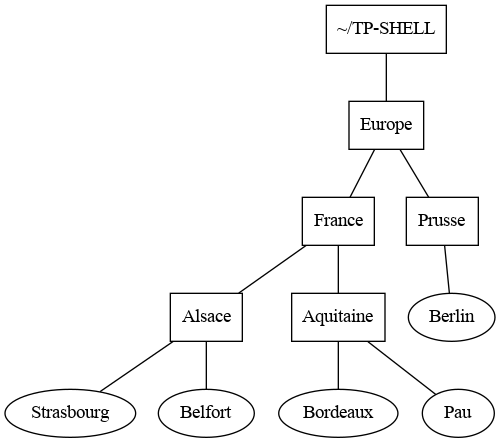
\includegraphics[width=0.6\textwidth,height=\textheight]{images/graphe-europe.png}\\

On se place dans le répertoire personnel de l'utilisateur représenté par
le raccourci \texttt{\textasciitilde{}}.

\begin{enumerate}
\def\labelenumi{\arabic{enumi}.}
\tightlist
\item
  Dans son répertoire personnel, créer le répertoire ̀̀\texttt{TP-SHELL}
  puis entrer dans ce répertoire.
\item
  Créer le répertoire \texttt{Europe} et changer de répertoire courant
  pour \texttt{Europe}.
\item
  Écrire une suite de commandes qui permet de construire l'arborescence
  ci-dessus sans quitter le répertoire \texttt{Europe}. Les fichiers
  apparaissant avec des rectangles sont des répertoires et les autres
  sont des fichiers.
\item
  Créer dans \texttt{\textasciitilde{}} une copie de tout le répertoire
  \texttt{Europe} avec ses sous-répertoires et nommer cette copie
  \texttt{Vieille-Europe}. Les modifications qui suivent devront être
  faites dans \texttt{Europe}.
\item
  Appliquons le traité de Francfort de 1871. Se placer dans le
  répertoire \texttt{Prusse} et déplacer \texttt{Belfort} dans
  \texttt{France} puis déplacer \texttt{Alsace} dans \texttt{Prusse}.
  Revenir dans \texttt{Europe} et renommer \texttt{Prusse}en
  \texttt{Allemagne}.
\item
  Depuis \texttt{Europe}, afficher le contenu de \texttt{Bordeaux} puis
  détruire ce fichier.
\item
  Appliquons le traité de Versailles de 1919. Depuis \texttt{France},
  ramener \texttt{Alsace} en \texttt{France} puis détruire
  \texttt{Vieille-Europe}.
\end{enumerate}

\end{exercice}

\hypertarget{exercices-plus-avancuxe9s}{%
\section{Exercices plus avancés}\label{exercices-plus-avancuxe9s}}

\hypertarget{flux-dentruxe9e-sortie-et-redirections-filtres-et-pipeline}{%
\subsection{Flux d'entrée / sortie et redirections, filtres et
pipeline}\label{flux-dentruxe9e-sortie-et-redirections-filtres-et-pipeline}}

\begin{methode}{}

\begin{itemize}
\item
  Par défaut, chaque programme (dont les commandes \emph{shell}) exécuté
  dans un \emph{shell} \href{https://fr.wikipedia.org/wiki/Unix}{UNIX}
  admet trois canaux, ou flux, de communication avec l'extérieur :

  \begin{itemize}
  \tightlist
  \item
    Un canal d'entrée nommé \emph{entrée standard} (\emph{stdin} en
    anglais) qui par défaut est le texte saisi au clavier dans le
    terminal.
  \item
    Un canal de sortie nommé \emph{sortie standard} (\emph{stdout} en
    anglais) qui par défaut est l'écran du terminal.
  \item
    Un canal d'erreur nommé \emph{erreur standard} (\emph{stderror} en
    anglais) qui par défaut est l'écran du terminal.
  \end{itemize}
\item
  On peut modifier l'entrée ou la sortie standard d'une comande pour
  lire ou écrire sur d'autres canaux que ceux par défaut (fichiers ou
  flux réseaux au lieu de clavier / écran ). Pour rediriger un flux vers
  l'entrée ou la sortie standard d'une commande on utilise des
  \emph{opérateurs de redirection} :
\end{itemize}

\begin{longtable}[]{@{}ll@{}}
\toprule
Opérateur & Redirection\tabularnewline
\midrule
\endhead
\textgreater{} & sortie standard\tabularnewline
\textgreater{}\textgreater{} & sortie standard en ajout à la
fin\tabularnewline
\textless{} & entrée standard\tabularnewline
\bottomrule
\end{longtable}

\begin{itemize}
\item
  Par exemple, si on veut écrire le contenu du répertoire courant dans
  un fichier \texttt{contenu.txt}, on redirige la sortie standard de
  \texttt{ls} vers un fichier \texttt{contenu.txt} au lieu de l'écran du
  terminal :

\begin{verbatim}
    junier@fredportable:~$ ls > contenu.txt
\end{verbatim}
\item
  Et si on veut compter le nombre de mots dans un texte, on redirige son
  entrée standard vers le contenu de \texttt{texte.txt} au lieu du
  clavier :

\begin{verbatim}
   junier@fredportable:~$ wc -m < texte.txt 
\end{verbatim}
\item
  On peut enchaîner les commandes en \emph{pipeline} : la sortie
  standard d'une commande est raccordée à l'entrée standard d'une
  commande suivante à l'aide d'un \emph{pip} symbolisé par le caractère
  \texttt{\textbar{}} :

\begin{verbatim}
      commande_debut | commande_fin
\end{verbatim}
\item
  Si on veut intercaler une commande entre les deux, elle doit envoyer
  son entrée standard sur sa sortie standard : de telles commandes qui
  servent de traitements intermédiaires entre le début et la fin d'un
  pipeline sont appelées \emph{filtres}. On peut ainsi réaliser en un
  une ligne de commande des traitements complexes.

\begin{verbatim}
      commande_debut | filtre1 | filtre2 | ... | commande_fin
\end{verbatim}
\item
  Le tableau ci-dessous donne quelques exemples de filtres, d'autres
  options sont disponibles pour chaque commande.
\end{itemize}

\end{methode}

\begin{longtable}[]{@{}ll@{}}
\toprule
\begin{minipage}[b]{0.13\columnwidth}\raggedright
Commande\strut
\end{minipage} & \begin{minipage}[b]{0.81\columnwidth}\raggedright
Action\strut
\end{minipage}\tabularnewline
\midrule
\endhead
\begin{minipage}[t]{0.13\columnwidth}\raggedright
cat\strut
\end{minipage} & \begin{minipage}[t]{0.81\columnwidth}\raggedright
copie son entrée standard sur sa sortie standard sans modification\strut
\end{minipage}\tabularnewline
\begin{minipage}[t]{0.13\columnwidth}\raggedright
sort\strut
\end{minipage} & \begin{minipage}[t]{0.81\columnwidth}\raggedright
trie les lignes de son entrée standard par ordre alphabétique\strut
\end{minipage}\tabularnewline
\begin{minipage}[t]{0.13\columnwidth}\raggedright
sort -r\strut
\end{minipage} & \begin{minipage}[t]{0.81\columnwidth}\raggedright
trie les lignes de son entrée standard par ordre alphabétique
inverse\strut
\end{minipage}\tabularnewline
\begin{minipage}[t]{0.13\columnwidth}\raggedright
sort -n\strut
\end{minipage} & \begin{minipage}[t]{0.81\columnwidth}\raggedright
trie les lignes de son entrée standard par ordre numérique\strut
\end{minipage}\tabularnewline
\begin{minipage}[t]{0.13\columnwidth}\raggedright
cut -d : -f 5\strut
\end{minipage} & \begin{minipage}[t]{0.81\columnwidth}\raggedright
sélectionne le 5 eme champ de chaque ligne de son entrée standard
découpée selon le délimiteur :\strut
\end{minipage}\tabularnewline
\begin{minipage}[t]{0.13\columnwidth}\raggedright
wc -l\strut
\end{minipage} & \begin{minipage}[t]{0.81\columnwidth}\raggedright
compte les lignes de son entrée standard\strut
\end{minipage}\tabularnewline
\begin{minipage}[t]{0.13\columnwidth}\raggedright
wc -w\strut
\end{minipage} & \begin{minipage}[t]{0.81\columnwidth}\raggedright
compte les mots de son entrée standard\strut
\end{minipage}\tabularnewline
\begin{minipage}[t]{0.13\columnwidth}\raggedright
wc -m\strut
\end{minipage} & \begin{minipage}[t]{0.81\columnwidth}\raggedright
compte les caractères de son entrée standard\strut
\end{minipage}\tabularnewline
\begin{minipage}[t]{0.13\columnwidth}\raggedright
uniq\strut
\end{minipage} & \begin{minipage}[t]{0.81\columnwidth}\raggedright
supprime les lignes considérées comme des doublons\strut
\end{minipage}\tabularnewline
\begin{minipage}[t]{0.13\columnwidth}\raggedright
head -n5\strut
\end{minipage} & \begin{minipage}[t]{0.81\columnwidth}\raggedright
affiche les cinq premières lignes de son entrée standard\strut
\end{minipage}\tabularnewline
\begin{minipage}[t]{0.13\columnwidth}\raggedright
head -n-5\strut
\end{minipage} & \begin{minipage}[t]{0.81\columnwidth}\raggedright
affiche tout sauf les cinq dernières lignes de son entrée standard\strut
\end{minipage}\tabularnewline
\begin{minipage}[t]{0.13\columnwidth}\raggedright
tail -n5\strut
\end{minipage} & \begin{minipage}[t]{0.81\columnwidth}\raggedright
affiche les cinq dernières lignes de son entrée standard\strut
\end{minipage}\tabularnewline
\begin{minipage}[t]{0.13\columnwidth}\raggedright
tail -n+5\strut
\end{minipage} & \begin{minipage}[t]{0.81\columnwidth}\raggedright
affiche tout sauf les cinq premières lignes de son entrée standard\strut
\end{minipage}\tabularnewline
\bottomrule
\end{longtable}

\includegraphics[width=0.5\textwidth,height=\textheight]{https://upload.wikimedia.org/wikipedia/commons/thumb/7/70/Stdstreams-notitle.svg/640px-Stdstreams-notitle.svg.png}\\

\begin{exercice}{}

\emph{Exercice du manuel de première NSI de Thibault Balabonski chez
Ellipses}

Le fichier \texttt{/etc/passwd} contient la liste des utilisateurs
locaux de la machine. Pour chaque question, on recherchera
éventuellement dans le manuel avec la commande \texttt{man\ command} les
options pertinentes des commandes proposées.

\begin{enumerate}
\def\labelenumi{\arabic{enumi}.}
\tightlist
\item
  Afficher les 5 premières lignes du fichier \texttt{/etc/passwd}.
\item
  Afficher la page du manuel de la commande \texttt{tac} puis utiliser
  cette commande pour afficher \texttt{tac} à l'envers.
\item
  Trier le fichier \texttt{/etc/passwd} avec la commande \texttt{sort}.
  Quel ordre est utilisé ?
\item
  Les champs de chaque ligne de \texttt{/etc/passwd} sont séparées par
  le caractère \texttt{:}. Trier le fichier selon le troisième champ.
  Quel ordre est utilisé ?
\item
  Trier \texttt{/etc/passwd} selon le troisième champ avec l'ordre
  numérique.
\end{enumerate}

\end{exercice}

\begin{exercice}{}

\begin{enumerate}
\def\labelenumi{\arabic{enumi}.}
\item
  Ouvrir un terminal \emph{shell} et choisir comme répertoire courant
  ̀\texttt{\textasciitilde{}/TP-SHELL}.
\item
  Créer un un répertoire \texttt{carnet} puis entrer dans ce répertoire.
\item
  Consulter l'aide de la commande \texttt{wget} avec
  \texttt{wget\ -\/-help} ou \texttt{man\ wget} puis télécharger le
  fichier
  d'\href{https://fr.wikipedia.org/wiki/Uniform_Resource_Locator}{URL} :
  \url{https://gitlab.com/frederic-junier/nsi-public/-/raw/master/Premiere/Systeme/TP2/contacts-1000.csv}
\item
  Afficher les 3 premières lignes de \texttt{contacts-1000.csv}, puis
  ses 3 dernières lignes puis son nombre de lignes. Chaque ligne
  contient un nom de contact et une adresse mail séparés par le
  caractère \texttt{,}.
\item
  Écrire une commande qui affiche les 10 premières lignes du contenu de
  \texttt{contacts-1000.csv} classé par ordre alphabétique croissant.
\item
  Écrire une commande qui trie \texttt{contacts-1000.csv} par ordre
  alphabétique croissant puis recopie ce contenu dans le fichier
  \texttt{contacts-1000-alpha.csv}.
\item
  Écrire une commande qui filtre les lignes de
  \texttt{contacts-1000.csv} en sélectionnant uniquement le champ nom
  puis qui classe ces noms par ordre alphabétique croissant.
\item
  Compléter la commande précédente pour qu'elle supprime les doublons et
  affiche devant chaque nom le nombre de doublons, c'est-à-dire
  d'adresses mails du contact. On consultera la page de manuel de la
  commande \texttt{uniq} pour sélectionner la bonne option.
\item
  Modifier la commande précédente pour que les contacts soient classés
  par nombre décroissant d'adresses mails et que le tout soit redirigé
  vers un fichier \texttt{top-mails.txt}.
\end{enumerate}

\end{exercice}

\hypertarget{recherches}{%
\subsection{Recherches}\label{recherches}}

\begin{methode}{}

Le \emph{shell}
\href{https://fr.wikipedia.org/wiki/Bourne-Again_shell}{BASH} fournit de
nombreuses commandes pour rechercher des informations dans le système de
fichiers.

\begin{itemize}
\tightlist
\item
  Pour une recherche sur les fichiers, on peut utiliser la commande
  \texttt{find} qui permet d'effectuer une recherche par nom parmi de
  nombreuses options :
\end{itemize}

\begin{longtable}[]{@{}ll@{}}
\toprule
\begin{minipage}[b]{0.23\columnwidth}\raggedright
Commande\strut
\end{minipage} & \begin{minipage}[b]{0.71\columnwidth}\raggedright
Action\strut
\end{minipage}\tabularnewline
\midrule
\endhead
\begin{minipage}[t]{0.23\columnwidth}\raggedright
find -name photo.png\strut
\end{minipage} & \begin{minipage}[t]{0.71\columnwidth}\raggedright
recherche les fichiers nommés photo.png dans le répertoire courant et
tous ses sous-répertoires\strut
\end{minipage}\tabularnewline
\begin{minipage}[t]{0.23\columnwidth}\raggedright
find -iname photo.png\strut
\end{minipage} & \begin{minipage}[t]{0.71\columnwidth}\raggedright
idem mais insensible à la casse\strut
\end{minipage}\tabularnewline
\begin{minipage}[t]{0.23\columnwidth}\raggedright
find -name photo.png \textasciitilde{}/sandbox\strut
\end{minipage} & \begin{minipage}[t]{0.71\columnwidth}\raggedright
recherche les fichiers nommés photo.png dans le répertoire
\textasciitilde{}/sandbox et tous ses sous-répertoires\strut
\end{minipage}\tabularnewline
\begin{minipage}[t]{0.23\columnwidth}\raggedright
find -name '*.png' \textasciitilde{}/sandbox\strut
\end{minipage} & \begin{minipage}[t]{0.71\columnwidth}\raggedright
recherche les fichiers dont le nom se termine par \texttt{.png} dans le
répertoire \textasciitilde{}/sandbox et tous ses sous-répertoires\strut
\end{minipage}\tabularnewline
\bottomrule
\end{longtable}

\begin{itemize}
\item
  Par exemple, si on veut rechercher le fichier `ducotedechezswann.txt'
  dans son répertoire personnel :

\begin{verbatim}
    junier@fredportable:~$ find -name 'ducotedechezswann.txt' 
    ./Git/Gitlab/frederic-junier/Premiere-NSI/ducotedechezswann.txt
    ./NSI/TP/ressources/ducotedechezswann.txt
\end{verbatim}
\item
  Pour une recherche sur un contenu de fichier, on peut utiliser la
  commande \texttt{grep} qui permet d'effectuer une recherche d'un
  fragment de texte dans les fichiers donnés en argument. Par défaut
  \texttt{grep} affiche chaque ligne de fichier où le fragment apparaît.
\end{itemize}

\begin{longtable}[]{@{}ll@{}}
\toprule
\begin{minipage}[b]{0.25\columnwidth}\raggedright
Commande\strut
\end{minipage} & \begin{minipage}[b]{0.69\columnwidth}\raggedright
Action\strut
\end{minipage}\tabularnewline
\midrule
\endhead
\begin{minipage}[t]{0.25\columnwidth}\raggedright
grep `fragment texte' fichier\strut
\end{minipage} & \begin{minipage}[t]{0.69\columnwidth}\raggedright
recherche les occurences de `fragment texte' dans fichier\strut
\end{minipage}\tabularnewline
\begin{minipage}[t]{0.25\columnwidth}\raggedright
grep -c `fragment texte' fichier\strut
\end{minipage} & \begin{minipage}[t]{0.69\columnwidth}\raggedright
affiche juste le nombre d'occurences de `fragment texte' dans
fichier\strut
\end{minipage}\tabularnewline
\begin{minipage}[t]{0.25\columnwidth}\raggedright
grep -r `fragment texte' rep\strut
\end{minipage} & \begin{minipage}[t]{0.69\columnwidth}\raggedright
recherche les occurences de `fragment texte' dans le répertoire rep et
tous ses sous-répertoires\strut
\end{minipage}\tabularnewline
\begin{minipage}[t]{0.25\columnwidth}\raggedright
grep -r -l -i `fragment texte' rep\strut
\end{minipage} & \begin{minipage}[t]{0.69\columnwidth}\raggedright
idem mais n'affiche que les noms de fichiers et insensible à la
casse\strut
\end{minipage}\tabularnewline
\bottomrule
\end{longtable}

\begin{itemize}
\item
  Par exemple si on veut compter le nombre d'occurences de `swann' dans
  le texte `unamourdeswann.txt' :

\begin{verbatim}
    junier@fredportable:~$ grep -i -c 'swann' ducotedechezswann.txt
    685
\end{verbatim}
\end{itemize}

\end{methode}

\begin{exercice}{}

Ouvrir un terminal avec la page de manuel de la commande \texttt{find}
obtenue avec \texttt{man\ find}.

Ouvrir un autre terminal pour traiter les questions suivantes.

\begin{enumerate}
\def\labelenumi{\arabic{enumi}.}
\item
  Écrire une commande qui affiche tous les fichiers d'extension
  \texttt{.py} contenus dans son répertoire personnel ou ses sous
  répertoires.
\item
  Compléter la commande précédente pour afficher le nombre des fichiers
  trouvés.
\item
  Compter de même le nombre de fichiers d'extension \texttt{.py} dans le
  répertoire \texttt{/usr/share}.
\item
  Écrire une commande qui compte le nombre total de répertoires contenus
  dans son répertoire personnel \texttt{\textasciitilde{}} et tous ses
  sous-répertoires.
\item
  Écrire une commande qui compte le nombre de fichiers qui ne sont pas
  des répertoires et qui ont été créés dans son répertoire personnel et
  tous ses sous-répertories dans les dix dernières minutes.
\end{enumerate}

\end{exercice}

\begin{exercice}{}

Le projet Gutenberg met à disposition des utilisateurs des textes du
domaine public en format numérique (\texttt{txt}, \texttt{epub}
\ldots{}) sous licence libre (voir
\href{https://www.gutenberg.org/wiki/Gutenberg:The_Project_Gutenberg_License}{The
Gutenberg License}).

Le texte brut du ``Tour du monde en 80 jours'' écrit par Jules Verne est
disponible à partir de
l'\href{https://fr.wikipedia.org/wiki/Uniform_Resource_Locator}{URL}
\url{http://www.gutenberg.org/ebooks/800.txt.utf-8}.

\begin{enumerate}
\def\labelenumi{\arabic{enumi}.}
\item
  Ouvrir un terminal \emph{shell} et choisir comme répertoire courant
  \texttt{\textasciitilde{}/TP-SHELL}.
\item
  Créer un un répertoire \texttt{Phileas} puis entrer dans ce
  répertoire.
\item
  Consulter l'aide de la commande \texttt{wget} avec
  \texttt{wget\ -\/-help} ou \texttt{man\ wget} puis télécharger le
  fichier contenant le texte du ``Tour du monde en 80 jours'' au format
  \texttt{txt}.

\begin{verbatim}
 junier@fredportable:~/TP-SHELL/Phileas$ ls
 800.txt.utf-8
\end{verbatim}
\item
  Renommer le fichier en \texttt{tour-du-monde-80-jours.txt}.

\begin{verbatim}
 junier@fredportable:~/TP-SHELL/Phileas$ ls
 tour-du-monde-80-jours.txt
\end{verbatim}
\item
  Afficher le nombre de lignes, le nombre de mots, le nombre de
  caractères et le nombre d'octets de
  \texttt{tour-du-monde-80-jours.txt} avec des options bien choisies de
  la commande \texttt{wc}. Comment peut-on expliquer que le nombre de
  caractères est inférieur au nombre d'octets ? Vérifier l'encodage du
  fichier avec la commande \texttt{file\ tour-du-monde-80-jours.txt}.
\item
  Les commandes \texttt{du} et \texttt{zip} permettent respectivement
  d'afficher la taille d'un fichier et de compresser un fichier.
  Consulter leurs pages de manuel avec
  \texttt{man\ du\ \textbar{}\ less} et
  \texttt{man\ zip\ \textbar{}~less}. La commande \texttt{less} est un
  \emph{pager} qui permet d'afficher une page à la fois dans le
  terminal.
\end{enumerate}

\begin{itemize}
\tightlist
\item
  Afficher la taille du fichier en kilo-octets avec la commande
  \texttt{du\ -h\ tour-du-monde-80-jours.txt}.
\item
  Compresser la fichier avec la commande \texttt{zip}. Quel est le taux
  de compression ?
\item
  Avec la commande \texttt{head}, afficher les dix premières lignes des
  fichiers \texttt{tour-du-monde-80-jours.txt} et
  \texttt{tour-du-monde-80-jours.zip}. Que peut-on remarquer ?
\end{itemize}

\begin{enumerate}
\def\labelenumi{\arabic{enumi}.}
\setcounter{enumi}{6}
\tightlist
\item
  Consulter la page de manuel de la commande \texttt{tac} avec
  \texttt{man\ \textbar{}~less\ tac}. En une seule commande, créer un
  fichier \texttt{tour-du-monde-80-jours-inverse.txt} où toutes les
  lignes du fichier initial sont recopiées à l'envers.
\item
  Dans \texttt{tour-du-monde-80-jours.txt}, avec la commande
  \texttt{grep} et des options bien choisies :
\end{enumerate}

\begin{itemize}
\tightlist
\item
  Compter le nombre d'occurences du mot \texttt{phileas}. On doit
  trouver 330.
\item
  Afficher le numéro de ligne du fragment de texte ``*** START OF''.
  Vérifier avec un éditeur de textes.
\item
  Afficher le numéro de ligne du fragment de texte ``*** END OF''.
  Vérifier avec un éditeur de textes.
\item
  En une seule commande, créer un fichier texte
  \texttt{tour-du-monde-80-jours-brut.txt} qui contient toutes les
  lignes comprises entre celles commençant par \texttt{***\ START\ OF}
  et \texttt{***\ END\ OF}, les deux bornes exclues.
\end{itemize}

\end{exercice}

\end{document}
